
\subsection*{task 1.4 [20 points] \\[1ex] finding maximally different images}

So far, you only had to do what the problem specifications asked you to do. In this task, you need to get creative!

Reread matrix $\mat{X}$ from task 1.1 into memory but \emph{do not normalize it to zero mean}. Now, think of / invent an algorithm that selects $k>2$ out of the $n$ columns of $\mat{X}$ such that the selected data vectors are as far apart as possible. 

Mathematically, the problem considered in this task is a subset selection problem and we can formalize it as follows: given $X = \{ \vec{x}_1, \ldots, \vec{x}_n \}$, solve
\begin{align*}
S^* = \amax{S \subset X} & \sum_{\vec{x}_i \in S} \sum_{\vec{x}_j \in S} \dsq{\vec{x}_i}{\vec{x}_j} \\
\st \; & \; \; \lvert S \rvert = k
\end{align*}
\textbf{NOTE:} this problem is actually way more difficult than it may appear at first sight; in fact, it is NP-complete and an \textit{efficient} algorithm that is \textit{guaranteed} to find the optimal $S^*$ for very large sets $X$ and arbitrary choices of $k$ remains elusive to this date. \vspace{1ex}

%%%%%
%%%%%
%%%%% enter your code into the following environment
%%%%%
%%%%%
\begin{python}
# past your code here
## Some helpers

# compute the objective function on a set
def obj_func(set):
    sum = 0;
    for s1 in set:
        for s2 in set:
            sum += np.linalg.norm(s1-s2,2)
    return sum


# images: array of images, that should be printed
# shape: width * height of output
# path: where the image should be stored to
def print_images(images, shape, path):
    width = shape[0]
    height = shape[1]
    if not len(images) == width * height:
         raise ValueError("wrong shape")
        
    fig, axes = plt.subplots(width, height)
    # remove the x and y ticks
    for i in range(width):
        for j in range(height):
            axes[i, j].imshow(images[i*width+j].reshape(19,19))
    plt.setp(plt.gcf().get_axes(), xticks=[], yticks=[]);
    fig.savefig(path)

# use k-means and choose k images that are near centroids
from scipy.cluster.vq import vq, kmeans, whiten

def findPointNearCentroid(centroid, points):
    # iterate through all points and find the nearest
    min_dif = np.infty
    point = None
    for p in points:
        dif = np.linalg.norm(p - centroid, 2)
        if dif < min_dif:
            point = p
            min_dif = dif
    return point
    

def approach1(N):    
    cluster = kmeans(mat, N)
    centroids = cluster[0]
    optimal_set = []

    for c in centroids:
        point = findPointNearCentroid(c, mat)
        optimal_set.append(point)
        
    return (optimal_set, obj_func(optimal_set))
    

\end{python}
%%%%%
%%%%%
%%%%%
%%%%%
%%%%%
\vspace{2cm}

Testing the algorithm for sizes 25, 50 and 100:
%%%%%
%%%%%
%%%%% enter your plots here, i.e. replace "t1-4-k*.png" by the names of the graphics files you created
%%%%%
%%%%%
\begin{center}
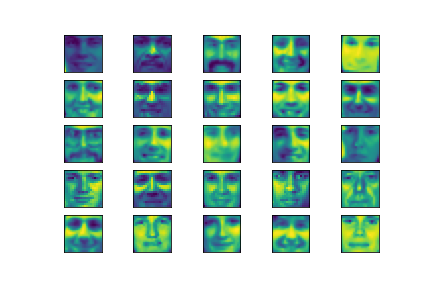
\includegraphics[width=1\textwidth]{Ex_01/Figures/t1-4-k4.png} 
\quad
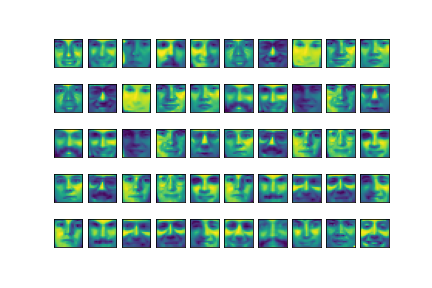
\includegraphics[width=1\textwidth]{Ex_01/Figures/t1-4-k9.png}
\quad
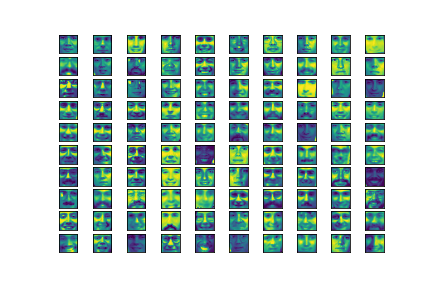
\includegraphics[width=1\textwidth]{Ex_01/Figures/t1-4-k16.png}
\end{center}
%%%%%
%%%%%
%%%%%
%%%%%
%%%%%







